\section{$(g-2)_\mu$ Discrepancy}
The $g$ factor of the magnetic moment of a particle describes the coupling between spin angular momentum and the magnetic moment of the particle.
Dirac shows that this factor is $g=2$ for the electron, and this also would extend to the muon.
However, loop corrections can give an additional effect that was not taken into account by Dirac.
Within the SM, it is expected that $a \equiv (g-2)/2 \neq 0$.
If we examine the QED vertex, we can see that it can be expanded as the bare vertex plus higher order loop diagrams.
One of these loop diagrams in particular corresponds to the magnetic moment being different than two and is seen in Fig.~\ref{fig:magnetic_moment}.

\begin{figure}[h]
    \centering
    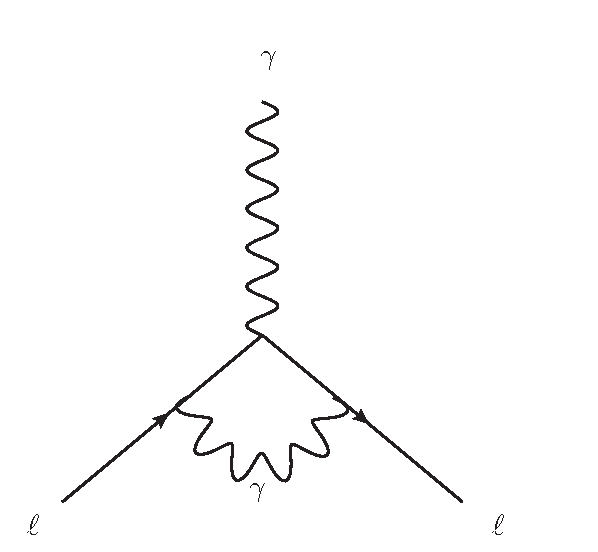
\includegraphics[width=0.4\textwidth]{Figures/feynman_diagrams/muon_magnetic_moment}
    \caption{Single loop diagram contributing to the magnetic moment of the leptons.}
    \label{fig:magnetic_moment}
\end{figure}

This diagram, when computed for the electron, yields a contribution to $a_e \equiv (g_e - 2)/2 = \frac{\alpha}{2\pi}$.
For the electron, this works very well and has precision down to 5 loops, which translates to 0.25 parts-per-billion \cite{Aoyama:2012wj}.
This is actually used to do precision QED tests, and we take this to be how we define $1/\alpha = 137.035999174(35)$.
The theory predicts $a_e = 1,159,652,181.78(77)\times 10^{-12}$, when using an alternative determination of $\alpha$, as $\alpha$ is usually extracted by precision measurements of $a_e$.

However, this does not seem to work for the muon, or at least not as precisely for the electron \cite{Jegerlehner:2009ry}.
The value of $a_\mu \equiv \frac{(g_\mu-2)}{2}$ was sought out at the Brookhaven E821 experiment in 2001, with their final result being delivered in 2004 \cite{Hagiwara:2006jt}.
They found that the true value is $a_\mu = 11,659,208.0(6.3)\times 10^{-10}$, yielding a difference of $\Delta a_\mu = (290\pm90)\times 10^{-11}$, a $3.4\sigma$ deviation between experiment and theory once the mass effects are taken into account \cite{Jegerlehner:2009ry}.
Note that $a_\mu$ has many components contributing to it, and can be split into the QED component, the EW component, and the hadronic component.
The first two are know to very good accuracy, but the hadronic component is naturally harder to compute.
Once these are all taken into account at leading order, or next to leading order, the expected theoretical value is $a_\mu = (11,659,180.4 \pm 5.1)\times 10^{-10}$, making it more clear that there is in fact a $3.4\sigma$ effect.

While this discrepancy is not huge, and may still be a result of a statistical fluctuation or an error, it could be a window into new physics.
Any new mediator that can be introduced in a loop similar to the magnetic and couples to leptons will change $a_\mu$ and $a_e$.
There is a wide variety of new physics options that have been investigated to solve the anomalous magnetic moment of the muon.
For example, it has been speculated that weak scale physics, such as light SUSY, could be responsible for the deviations in $a_\mu$ \cite{Czarnecki:2001pv}.
In particular, one model that has been examined quite extensively in this regard is the dark photon.
The parameter space allows for a narrow band that could explain $a_\mu$ without disturbing $a_e$, since the mass may be too large to have an effect as a loop with electrons on the legs.
Recently, these points in the parameter space have been excluded by kaon decay at NA48/2, so it may appear that the dark photon can not explain the $a_\mu$ discrepancy~\cite{Batley:2015lha}.
We will discuss kaon decay in more detail later on in the thesis.

A recent effort at Fermilab has been taken to remeasure $(g-2)_\mu$, in the E989 experiment \cite{Venanzoni:2014ixa}.
The expected result is a decrease in the uncertainty by a factor of four, reaching a precision of $0.14$ ppm.
There are also attempts to calculate $a_\mu$ more precisely with lattice QCD \cite{Juttner:2009yb, Renner:2010zj, Malak:2015sla}.
Calculating using the lattice could minimize the uncertainties from the theory side.
